\section{Конструкторская часть}

\subsection{Разработка алгоритма}
Ниже, на рисунке \ref{tab:1}, приведен алгоритм для «умного» светофора, , сделанны студентом Динь Вьет Ань.

\begin{figure}[H]
	\begin{center}
		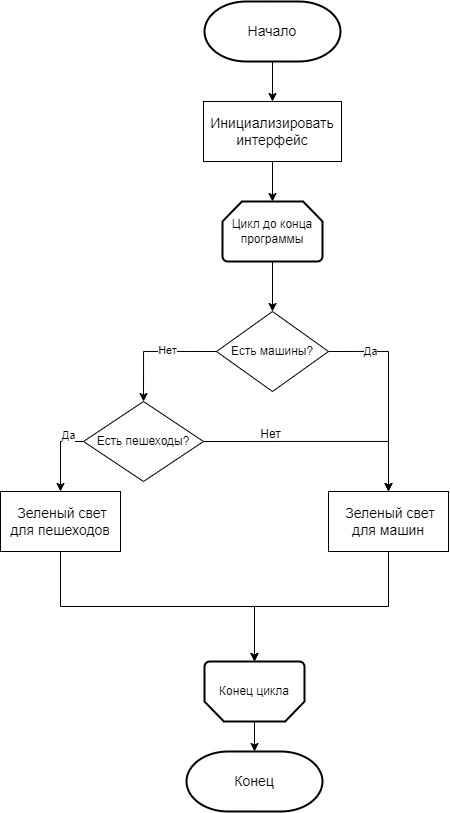
\includegraphics[scale=0.7]{img/al.jpg}
	\end{center}
	\captionsetup{justification=centering}
	\caption{Aлгоритм для «умного» светофора.}
	\label{img:s14}
\end{figure}
\subsection{Структура и состав классов}

В программе имеет следующие классы:
\begin{itemize}[label = ---]
    \item Program --- входная точка в программу; 
    \item Form --- класс интерфейса;
    \item trafficlight --- сохранит информации о системе светофоров для машин, методы преобразования цвета светофора для машин;;
    \item pedestrialight --- сохранит информации о системе светофоров для пешеходов, методы преобразования цвета светофора для пешеходов;
    \item car --- сохранит информации о машинах.
\end{itemize}